\subsection{Perimeter}
\subsubsection{Circle}
$$ 2 \pi r $$

\subsection{Areas}
\subsubsection{Circle}
$$ \pi r^2 $$
\subsubsection{Triangle}
$$ \dfrac{b * h}{2} $$
\subsubsection{Square}
$$ l^2 $$
\subsubsection{Rectangle}
$$ hr $$
\subsubsection{Rhombus}
\begin{center}
    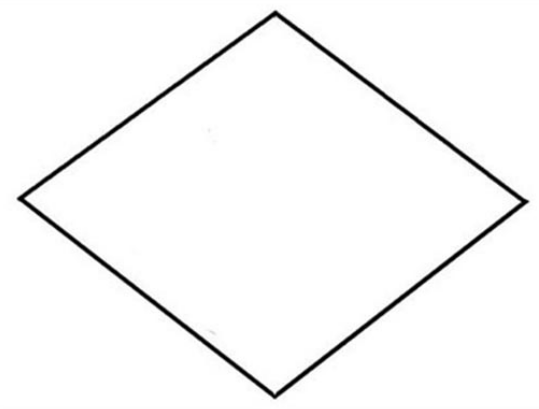
\includegraphics[scale=.2, keepaspectratio]{./Theory/images/rhombus.png}
\end{center}
$D$ is the biggest diagonal and $d$ is the smallest diagonal
$$ A = \dfrac{1}{2} * D * d $$
\subsubsection{Circular Sector}
\begin{center}
    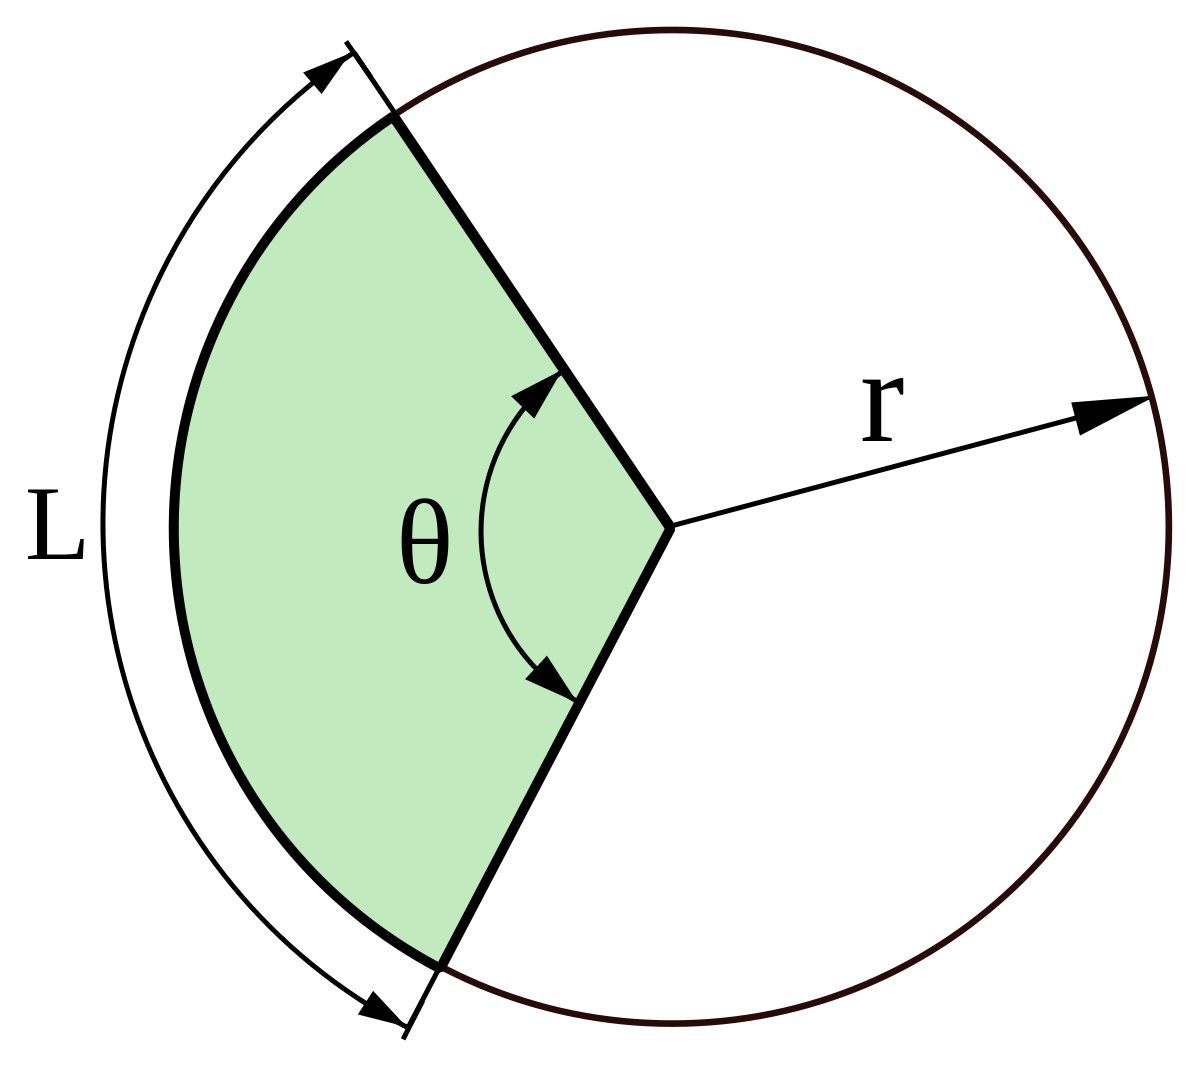
\includegraphics[scale=.2, keepaspectratio]{./Theory/images/circularsector.png}
\end{center}

$$ A = \dfrac{l * d}{2} $$

For $\alpha$ in radians:
$$ A = \dfrac{r^{2} * \alpha}{2} $$

For $\theta$ in degrees:
$$ A = \dfrac{\theta * \pi * r^{2}}{360^{\circ}} $$

\subsection{Volumes}
\subsubsection{Sphere}
$$ \dfrac{4}{3} \pi r^3 $$
\subsubsection{Prism}
$$ V = b h $$
\subsubsection{Pyramid}
$$ \dfrac{bh}{3} $$
\subsubsection{Cone}
$$ \dfrac{\pi r^2 h}{3} $$
